%% ============================================================================
%% EEM4011 -- Q1 MAKALE İSKELETİ (Elsevier: elsarticle)
%% Kimler için: Biomedical Signal Processing and Control, Computers in Biology and Medicine,
%%   Computer Methods and Programs in Biomedicine, Computerized Medical Imaging and Graphics ...
%% Kullanım: zip dosyasını Overleaf'e yükleyiniz (New project -> Existing project (.zip)); derleyici pdfLaTeX; Recompile.
%% ÖNCE DERGİ (HAFTA 1-A): sınırlar (kelime, özet, highlights, beyanlar) derginin "Guide for Authors"
%%   sayfasından alınır; aşağıdaki sayılar tipik değerlerdir, derginizinki farklı olabilir.
%% Haftalar: HAFTA 1-A dergi · 1-B katkı · 2-A Giriş · 2-B Yöntem · 3-A deney planı · 3-B Sonuçlar ·
%%   4-A şekil ve tablo · 4-B Tartışma · 5-A ön yüz ve beyanlar · 5-B gönderim öncesi denetim.
%% HAFTA 5-B: gönderimden önce KONTROL.md listesini uygulayınız; deneme hakemliğine derlenmiş PDF'i yükleyiniz.
%% Dosyalar: main.tex (ön yüz + beyanlar) | govde.tex (bölümler) | ortak_baslik.tex (paketler)
%%   sonuclar.csv + veri_ozeti.csv -> sonuc_uret.py -> sonuclar.tex | sekil_uret.py -> sekiller/Figure_2.pdf
%%   refs.bib | highlights.txt | KONTROL.md
%% DİKKAT: bu dosya yalnız ön yüzü ve beyanları içerir; bölümler govde.tex dosyasındadır. Makaleyi birine
%%   okutacaksanız (deneme hakemliği dahil) main.tex dosyasını değil, derlenmiş PDF'i veriniz.
%% ============================================================================
\documentclass[preprint,12pt]{elsarticle}   %% gönderim biçimi: tek sütun. Hakem sürümü için: review
%% Sayfa sınırı olan dergide SON düzeni bir kez deneyiniz: \documentclass[final,5p,times,twocolumn]{elsarticle}
\biboptions{numbers,sort&compress}
\usepackage{lineno}
%% ortak_baslik.tex -- iki iskelette de aynı: paketler, \sonuc makrosu, örnek uyarısı.
\usepackage[T1]{fontenc}
\usepackage{amsmath}
\usepackage{graphicx}
\graphicspath{{sekiller/}{./}}   %% şekil sekiller/ klasöründe ya da kökte (düz gönderim zip'i) bulunur
\usepackage{booktabs}
\usepackage{tabularx}
\usepackage{algorithm}
\usepackage{algpseudocode}
\usepackage{tikz}
\usetikzlibrary{positioning}
\usepackage{url}

%% --- Sonuç makroları: \sonuc{anahtar}. Değer yoksa PDF'te kalın "??anahtar" çıkar (sessiz geçmez). ---
\makeatletter
\newcommand{\sonucyaz}[2]{\expandafter\gdef\csname sonuc@#1\endcsname{#2}}
\newcommand{\sonuc}[1]{\@ifundefined{sonuc@#1}{\textbf{??\detokenize{#1}}}{\csname sonuc@#1\endcsname}}
\makeatother
% OTOMATİK ÜRETİLDİ (sonuc_uret.py) -- elle değiştirmeyiniz; sonuclar.csv değişince yeniden üretiniz.
\sonucyaz{kat.n}{10}
\sonucyaz{base.ort}{0.704}
\sonucyaz{base.ss}{0.016}
\sonucyaz{yeni.ort}{0.770}
\sonucyaz{yeni.ss}{0.023}
\sonucyaz{fark.ort}{0.066}
\sonucyaz{fark.alt}{0.054}
\sonucyaz{fark.ust}{0.078}
\sonucyaz{fark.p}{= 0.002}
\sonucyaz{fark.ptest}{exact}
\sonucyaz{fark.npos}{10}
\sonucyaz{yayin.ort}{0.773}
\sonucyaz{yayin.ss}{0.019}
\sonucyaz{yfark.ort}{\ensuremath{-}0.003}
\sonucyaz{yfark.alt}{\ensuremath{-}0.008}
\sonucyaz{yfark.ust}{0.002}
\sonucyaz{yfark.p}{= 0.256}
\sonucyaz{yfark.ptest}{exact}
\sonucyaz{yfark.npos}{4}
\sonucyaz{veri.kayit}{400}
\sonucyaz{veri.kisi}{100}
\sonucyaz{veri.fs}{2000}
   %% sonuc_uret.py üretir (elle doldurulmaz); başka yerde sonuç sayısı yazılmaz

%% --- Örnek uyarısı: kendi metninizi yazınca govde.tex'in başındaki \ornekuyarisi satırını siliniz. ---
\newcommand{\ornekuyarisi}{\par\noindent\fbox{\parbox{\dimexpr\linewidth-2\fboxsep-2\fboxrule}{\footnotesize
\textbf{ÖRNEK İSKELET.} Bu belgedeki cümleler ve sayılar yalnız biçimi göstermek içindir; gerçek
bir çalışmanın sonucu değildir. Kendi verinizle değiştiriniz, sonra bu kutuyu siliniz.}}\par\medskip}

\newenvironment{genistablo}{\begin{table}[t]}{\end{table}}   %% tek sütun: normal tablo

\journal{Journal of Dentistry}   %% HAFTA 1-A: hedef dergi (yedek: Diagnostics, MDPI). Kart: makale/DERGI_KARTI.md
%% Journal of Dentistry kılavuzu (25.11.2026): Original Research Report en çok ~20 sayfa (şekil ve tablo dahil);
%%   özet en çok 250 kelime, atıf yok; 1-7 anahtar kelime; highlights 3-5 madde, <=85 karakter (önerilir);
%%   ÇİFT KÖR hakemlik: gönderim sürümünde ad, kurum, teşekkür ve depo linki bu dosyadan çıkar, başlık sayfası ayrı dosya.

\begin{document}
\begin{frontmatter}   %% başlık, yazar, özet, anahtar kelimeler bu ortamın İÇİNDE olmalıdır

%% HAFTA 5-A -- Başlık: en çok ~15 kelime; nesne + yöntem + neyin ölçüldüğü. Kısaltma ve "novel" yok.
\title{Subject-wise Evaluation of a Simple Classifier for Abnormal Heart Sound Screening}

%% Yazarlar: öğrenci + danışman(lar). Adres ve e-posta kurumunuzunki olmalıdır.
%% Dergi çift kör hakemlik istiyorsa (dergi kartınız) ad, kurum ve kendi çalışmanıza atıflar gönderim sürümünde gizlenir.
\author[kku]{Ad Soyad\corref{cor1}}
\ead{e-posta@kurum.edu.tr}
\author[kku]{Danışman Ad Soyad}
\cortext[cor1]{Corresponding author}
\affiliation[kku]{organization={Department of Electrical and Electronics Engineering, University Name},
                  city={City}, country={Country}}

%% HAFTA 5-A -- Özet: TEK paragraf, derginin sınırı (çoğu Elsevier dergisinde en çok 250 kelime), atıf yok,
%% tanımsız kısaltma yok. Sıra: (1) problem (2) amaç (3) veri ve yöntem, sayılarıyla (4) ana sonuç, aralıkla
%% (5) koşul/sınır (6) tek cümlelik anlam. Sayılar \sonuc ile. Olumsuz ya da belirsiz sonucu da yazınız.
%% Gönderim sistemindeki özet kutusuna PDF'teki metni kopyalayınız (\sonuc makrosu yapıştırmayınız).
%% YÖN: 'rose', 'improved' gibi kelimeleri sonucunuzun yönüne göre seçiniz; düşük değeri iyi olan metrikte (MAE, RMSE)
%% sonuc_uret.py'de IYI_YON = -1 yapınız ve 'fell', 'had a lower error' gibi yazınız (fark.ort o zaman eksidir).
\begin{abstract}
Automated analysis of heart sounds could support screening, but reported performance depends
on how recordings are split between training and testing. This study compares a
single-feature rule with a logistic-regression classifier under a strictly subject-wise
protocol. We used \sonuc{veri.kayit} recordings from \sonuc{veri.kisi} subjects of an open
database and evaluated the rule, the classifier and one re-run published method on the same
\sonuc{kat.n} folds. Balanced accuracy rose from \sonuc{base.ort} for the rule to \sonuc{yeni.ort}
for the classifier; the mean paired difference was \sonuc{fark.ort} (95\% confidence interval
\sonuc{fark.alt} to \sonuc{fark.ust}, paired sign-flip test $p \sonuc{fark.p}$). The classifier
did not differ clearly from the published method (difference \sonuc{yfark.ort}, 95\% confidence
interval \sonuc{yfark.alt} to \sonuc{yfark.ust}). The result holds for one database and one
assignment of subjects to folds. A transparent classifier is therefore a reasonable
baseline-level reference, not an improvement over published methods, under subject-wise evaluation.
\end{abstract}
%% Dergi YAPILANDIRILMIŞ özet istiyorsa (ör. CMPB) yukarıdaki paragrafı derginin başlıklarına bölünüz:
%% \textbf{Background and Objective:} ... \textbf{Methods:} ... \textbf{Results:} ... \textbf{Conclusions:} ...

%% Highlights AYRI dosyadır (highlights.txt): 3-5 madde, her biri boşluklar dahil en çok 85 karakter, sonuç sayısı yok.

\begin{keyword}   %% 1-7 anahtar kelime; başlıktaki kelimeleri tekrar etmeyen, aranabilir terimler
heart sound \sep phonocardiogram \sep subject-wise cross-validation \sep balanced accuracy \sep screening
\end{keyword}

\end{frontmatter}

%% \linenumbers   %% dergi satır numarası istiyorsa açınız

%% ============================================================================
%% govde.tex -- makalenin GÖVDESİ (iki iskelette de aynı dosya; sınıf farkı main.tex'te).
%% Her bölümün başında: hangi HAFTA (rehberdeki hafta ve bölüm, ör. HAFTA 2-A) ve ne yazılacağı.
%% İngilizce örnek cümleler NÖTR bir konudan (kalp sesi) alınmıştır: kendi projenizle DEĞİŞTİRİNİZ.
%% Kural 1: Sonuç sayısı metne elle yazılmaz -> \sonuc{anahtar}. PDF'te "??" görüyorsanız o sayı eksiktir.
%% Kural 2: Her şekil, tablo, denklem ve algoritma metinde \ref ile anılır.
%% Kural 3: Yapay zekâ çıktısını olduğu gibi yapıştırmayınız; kontrol edip yalnız farkı alınız.
%% Kural 4: Yorum ve sonuç cümleleri sizindir. Bu derste şekil ve görüntü yapay zekâya ürettirilmez; sohbet yalnız
%%   sizin çizim ve diyagram kodunuzu düzeltebilir. Düzelttirdiyseniz beyan edilir: Elsevier'de diyagramın ALTYAZISINA,
%%   veri grafiğinde METHODS'a aracın adı, sürümü ve geliştiricisi yazılır; IEEE'de Acknowledgment'a; ayrıca HAFTA 5-A'daki beyana.
%% ============================================================================

\ornekuyarisi  %% <-- kendi metninizi yazınca bu satırı siliniz (1. sayfadaki uyarı kutusu kalkar)

%% ---------------------------------------------------------------------------
%% 1 INTRODUCTION  (HAFTA 2-A; katkı cümlesi ve iddia tablosu HAFTA 1-B'den gelir)   ~800-1000 kelime
%% Paragraf sırası: (1) problem neden önemli  (2) ne biliniyor (atıflı, yöntem aileleri hâlinde)
%% (3) eksik ne (tek, net cümle)  (4) Tablo 1  (5) katkılar (3 madde)  (6) yol haritası.
%% ---------------------------------------------------------------------------
\section{Introduction}
\label{sec:intro}

Cardiac auscultation is a low-cost first examination, and automated analysis of heart sound
recordings could support screening where specialists are scarce~\cite{Liu2016}.
%% (1) Bağlam: 2-3 cümle, her cümle atıflı (önem cümlesi de kaynak ister). Tıbbi iddia yazmayınız: "diagnoses" değil, "may support screening".

Open databases and public challenges have made algorithms comparable. A large open collection of
heart sound recordings was assembled for the 2016 PhysioNet/Computing in Cardiology
Challenge~\cite{Liu2016,Clifford2016}; the leading entries combined hand-crafted
features with learned representations~\cite{Potes2016}. More recent data add murmur annotations
at several auscultation locations and release a subject identifier with every
recording~\cite{Oliveira2022,Reyna2023}.
%% (2) Bilinenler: her cümlenin sonunda atıf; kaynakları tek tek değil, AİLE hâlinde anlatınız.
%% Kaynakçanın toplamı 25-40 kaynak; yarıdan fazlası son beş yıldan, en az üçü HEDEF derginin son üç yılından olmalıdır.

A recurring methodological concern in clinical machine learning is how the data are split:
when recordings of the same person appear in both training and test sets, the reported
performance overestimates what a new patient would obtain~\cite{Saeb2017}. Whether a simple,
transparent classifier keeps its advantage over a single-feature rule under a strictly
subject-wise protocol has not been reported for this task with paired statistics.
%% (3) Eksik (gap): TEK ve ölçülebilir. "Not been studied" demek için Tablo 1'deki satırlar kanıttır.

Table~\ref{tab:related} summarises the closest studies and what each leaves open.

\begin{genistablo}
\caption{Closest related work and the gap addressed here. \emph{(Example rows: replace with the
5--7 studies closest to your own project; every row needs a DOI in \texttt{refs.bib}.)}}
\label{tab:related}
\centering
\footnotesize
\begin{tabularx}{\linewidth}{@{}p{0.19\linewidth}p{0.25\linewidth}p{0.21\linewidth}X@{}}
\toprule
Study & Data and task & Approach & Left open for this problem \\
\midrule
Clifford et al.~\cite{Clifford2016} & 2016 challenge data~\cite{Liu2016}; normal vs.\ abnormal recording & Challenge overview of submitted classifiers & Hidden-test ranking; no paired comparison with a simple rule \\
Potes et al.~\cite{Potes2016} & Same 2016 challenge data & Ensemble of a feature-based and a deep-learning classifier & Complex model; effect of the split protocol not isolated \\
Oliveira et al.~\cite{Oliveira2022} & Paediatric data set with murmur and outcome labels and subject identifiers & Data descriptor & A data resource, not a method comparison \\
Reyna et al.~\cite{Reyna2023} & Challenge on the data of~\cite{Oliveira2022} & Challenge overview & Ranking of models on hidden data; no simple rule paired with them \\
Saeb et al.~\cite{Saeb2017} & Clinical machine learning in general & Record-wise vs.\ subject-wise cross-validation & Principle shown on other signals, not on heart sounds \\
\midrule
\textbf{This work} & Subset of the data of~\cite{Oliveira2022} & Single-feature rule vs.\ logistic regression; one published method re-run & Subject-wise, paired, with interval and test \\
\bottomrule
\end{tabularx}
\end{genistablo}
%% genistablo: elsarticle'da normal tablo, IEEEtran'da iki sütuna yayılan tablo (main.tex'te tanımlı).

The contributions of this study are:
\begin{itemize}
  \item A paired, subject-wise comparison of a single-feature rule, a logistic-regression
        classifier and a re-run published method on the same \sonuc{kat.n} folds.
  \item An estimate of the improvement in balanced accuracy with a 95\% confidence interval
        and a paired permutation test, rather than a single split.
  \item A scripted pipeline that produces all reported values from a single results file,
        released with the code.
\end{itemize}
%% Katkı maddeleri: isimle başlar ("A ...", "An ..."), ölçülebilir, "novel/efficient" gibi sıfat YOK.
%% Her madde iddia tablonuzdaki (HAFTA 1-B) bir satıra karşılık gelir.
%% EN YAKIN ÇALIŞMA (HAFTA 2-A): projenizin dayandığı YAYIMLANMIŞ çalışmayı adıyla anınız; ondan NEYİ AYNEN ALDIĞINIZI
%% ve ona NEYİ EKLEDİĞİNİZİ iki cümleyle yazınız. Ders raporunuz ve 2209-A başvurunuz yayımlanmamıştır; kaynak gösterilmez.

The paper is organised as follows. Section~\ref{sec:methods} describes the data, the
methods and the evaluation protocol. Section~\ref{sec:results} reports the results.
Section~\ref{sec:discussion} discusses them and states the limitations, and
Section~\ref{sec:conclusion} concludes.

%% ---------------------------------------------------------------------------
%% 2 MATERIALS AND METHODS  (HAFTA 2-B; 'Evaluation protocol and statistics' alt bölümü HAFTA 3-A)   ~1200-1600 kelime
%% Ölçüt: başka bir mühendis YALNIZ bu bölümü okuyarak çalışmayı tekrarlayabilmeli.
%% Bu bölümü KODUNUZ AÇIKKEN yazınız: metin, kodun gerçekten yaptığını anlatır.
%% ---------------------------------------------------------------------------
\section{Materials and Methods}
\label{sec:methods}

Figure~\ref{fig:pipeline} shows the processing chain; one pass of the chain is one
cross-validation fold. Table~\ref{tab:notation} lists the notation and
Table~\ref{tab:params} every setting used.

\begin{figure}[t]
\centering
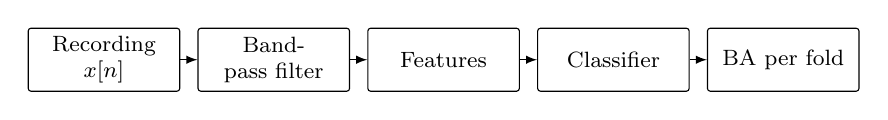
\begin{tikzpicture}[font=\footnotesize, node distance=0.018\linewidth,
  kutu/.style={draw, rounded corners=1pt, minimum height=8mm, text width=0.15\linewidth, align=center, inner sep=1.5pt}]
  \node[kutu] (a) {Recording $x[n]$};
  \node[kutu, right=of a] (b) {Band-pass filter};
  \node[kutu, right=of b] (c) {Features};
  \node[kutu, right=of c] (d) {Classifier};
  \node[kutu, right=of d] (e) {BA per fold};
  \foreach \u/\v in {a/b,b/c,c/d,d/e} \draw[-latex] (\u) -- (\v);
\end{tikzpicture}
\caption{Processing chain. The same chain is run for each of the three methods on each of the
\sonuc{kat.n} subject-wise folds.}
\label{fig:pipeline}
\end{figure}
%% Blok diyagram (Şekil 1): yöntemin tamamı tek bakışta. Altyazı "bir geçiş nedir, kaç kez tekrarlanır" der.
%% Diyagramı bu TikZ örneğinden kendiniz uyarlayınız; sohbet yalnız sizin kodunuzu düzeltebilir.

\subsection{Data}
\label{sec:data}
We used \sonuc{veri.kayit} recordings from \sonuc{veri.kisi} subjects of the CirCor DigiScope
data set (version~1.0.3, Open Data Commons Attribution License~v1.0)~\cite{Oliveira2022,Oliveira2022data},
obtained from PhysioNet~\cite{Pollard2026}. The data set releases a subject identifier with
every recording, which makes subject-wise splitting possible; the clinical outcome label
(normal or abnormal) released for each subject was used as the reference. All recordings were
resampled to \sonuc{veri.fs}~Hz.
%% Veri: adı, SÜRÜMÜ, LİSANSI, kayıt ve KİŞİ sayısı, veri veriyorsa yaş, cinsiyet ve sınıf dağılımı, dahil etme/çıkarma
%% ölçütü, etiketin kaynağı. Kişi (hasta) kimliği veride YOKSA "subject-wise" yazmayınız; durumu Limitations'a yazınız.
%% Aynı kişinin iki kimliği olabilir (bu veride iki taramaya katılanlar için "Additional ID"); bölmeden önce birleştiriniz.
%% Veri setini, deponun "please cite" metnindeki biçimde atıflayınız. Sayılar veri_ozeti.csv'den gelir: örnek değerleri
%% (400, 100, 2000) kendi verinizinkiyle değiştiriniz; değiştirmezseniz PDF'te örnek sayılar hata vermeden görünür.

\begin{table}[t]
\caption{Notation.}
\label{tab:notation}
\centering
\footnotesize
\begin{tabularx}{\linewidth}{@{}lXl@{}}
\toprule
Symbol & Meaning & Unit \\
\midrule
$x[n]$ & Heart sound recording, sample index $n$ & a.u. \\
$f_\mathrm{s}$ & Sampling rate & Hz \\
$K$ & Number of subject-wise folds & -- \\
$\mathit{Se}_k$, $\mathit{Sp}_k$ & Sensitivity and specificity on fold $k$ & -- \\
$\mathit{BA}_k$ & Balanced accuracy on fold $k$, Eq.~\eqref{eq:ba} & -- \\
$d_k$ & Paired difference (proposed minus baseline) on fold $k$ & -- \\
\bottomrule
\end{tabularx}
\end{table}
%% Notasyon tablosu İLK denklemden önce gelir. Her simgenin tek anlamı, bir birimi vardır.

\subsection{Baseline, published method and proposed method}
\label{sec:method}
The baseline labels a recording as abnormal when one spectral feature exceeds a threshold
chosen on the training folds. The proposed method feeds a small feature vector to a logistic
regression classifier. As an external reference, one published method~[CITE] was re-run with
its released code. All three use the same filtered signal and the same folds.
%% Baseline = en yalın, herkesin kabul edeceği yöntem. YAYIMLANMIŞ YÖNTEM = atıflı ve kodu açık bir yöntem;
%% AYNI katlarda yeniden koşunuz ve [CITE] yerine atfını yazınız (\cite{anahtar}). Yapmadıysanız bu cümleyi
%% ve sonuç tablosundaki satırı siliniz, nedenini Limitations'a yazınız; yapılmamış işi yazmayınız.
%% Kendi tanımladığınız bir skoru ya da eşiği yerleşik bir terimin adıyla sunmayınız: "score" ya da "index"
%% deyiniz, formülünü ve her parametresinin gerekçesini yazınız.

%% HAFTA 3-A: bu alt bölüm DENEY_PLANI.md dosyasından yazılır (plandan sapmalar dahil).
\subsection{Evaluation protocol and statistics}
\label{sec:protocol}
Performance is measured by the balanced accuracy on each fold $k$,
\begin{equation}
  \mathit{BA}_k = \tfrac{1}{2}\left(\mathit{Se}_k + \mathit{Sp}_k\right),
  \label{eq:ba}
\end{equation}
where $\mathit{Se}_k$ and $\mathit{Sp}_k$ are the sensitivity and specificity on the test
subjects of fold $k$. Equation~\eqref{eq:ba} is used instead of plain accuracy because the
two classes are imbalanced; it ranges from 0 to 1, and 0.5 corresponds to chance.
%% Her denklemden sonra: (a) simgeler, (b) denklemin NE İŞE yaradığı, (c) değer aralığı.
%% METRİK GÖREV TÜRÜNE GÖRE SEÇİLİR (rehber, Hafta 3, madde 2): sınıflandırma -> Se, Sp, dengeli doğruluk ya da F1;
%% olay tespiti -> tolerans penceresi içinde Se ve +P; kestirim -> birimli MAE/RMSE, bias ve %95 uyum sınırları;
%% bölütleme -> görüntü başına Dice ve IoU (medyanıyla). Sınıflandırmada karışıklık matrisi, ROC-AUC ve sınıf dengesi de verilir.
%% Alanınızın standardı ya da referans cihazı varsa sonucu ona göre de yazınız.

Folds are formed by subject (Algorithm~\ref{alg:cv}), so that no subject contributes to both
training and test data~\cite{Saeb2017}. We report the mean and standard deviation of
$\mathit{BA}_k$ over the $K$ folds, the mean paired difference $d_k$ with a 95\% bootstrap
confidence interval, and a paired sign-flip permutation test (exact for $n \le 16$, otherwise
100\,000 random sign flips; here: \sonuc{fark.ptest}) at a significance level of 0.05. Folds
share training data, so fold-wise results are not independent and the interval and the test
are approximate. All statistics are computed by the released script from one results file.
%% İstatistik: ortalama + yayılım + (aralık ya da test). Testin ADI ve yazılımı burada yazılır.
%% Başarı/başarısızlık eşikleri, sonuçlar GÖRÜLMEDEN önce burada sayıyla tanımlanır.
%% Katlar eğitim verisini paylaşır: mümkünse her TEST KİŞİSİ için bir satır üretiniz (n = kişi sayısı; sınıflandırmada
%% doğru 1, yanlış 0). Kat bazlı kalırsa en az 10 kat kullanınız (5 katta tam testin verebileceği en küçük p 0,0625'tir);
%% yukarıdaki "approximate" cümlesi ve Limitations'taki karşılığı metinde kalmalıdır. n'yi neden seçtiğinizi yazınız.
%% Sonuçları planı yazmadan önce gördüyseniz eşiği "önceden belirlenmiş" gibi sunmayınız (HAFTA 3-A).

\begin{algorithm}[t]
\caption{Subject-wise $K$-fold evaluation (run once per method)}
\label{alg:cv}
\begin{algorithmic}[1]
\Require recordings with subject identifiers, number of folds $K$, random seed
\State Assign every \emph{subject} to one of $K$ folds using the seed
\For{$k = 1, \dots, K$}
  \State Train on all recordings of subjects outside fold $k$
  \State Choose thresholds and hyper-parameters on the training data only
  \State Predict the recordings of subjects in fold $k$; compute $\mathit{Se}_k$, $\mathit{Sp}_k$, $\mathit{BA}_k$
\EndFor
\State \Return $\mathit{BA}_1, \dots, \mathit{BA}_K$ \Comment{one row per fold in \texttt{sonuclar.csv}}
\end{algorithmic}
\end{algorithm}
%% Algoritma kutusu: metinde bir cümleyle anlatınız ("Algorithm 1 assigns ..."); kutu metnin yerine geçmez.

\begin{table}[t]
\caption{Experimental settings. \emph{(Example: list every value a reader needs to repeat the study.)}}
\label{tab:params}
\centering
\footnotesize
\begin{tabularx}{\linewidth}{@{}lX@{}}
\toprule
Setting & Value \\
\midrule
Recordings / subjects & \sonuc{veri.kayit} / \sonuc{veri.kisi} \\
Sampling rate after resampling & \sonuc{veri.fs}~Hz \\
Band-pass filter & 4th-order Butterworth, 25--400~Hz \\
Cross-validation & subject-wise, $K=\sonuc{kat.n}$, seed 2026 \\
Classifier & logistic regression, default regularisation \\
Software & Python 3.12, NumPy~\cite{Harris2020}, SciPy~\cite{Virtanen2020} \\
Hardware and run time & laptop CPU, 16~GB RAM; about 2~s per fold \\
Code version & tag \texttt{v1.0} of the code repository \\
\bottomrule
\end{tabularx}
\end{table}
%% Parametre tablosu: filtre, pencere, eşik, tohum (seed), yazılım SÜRÜMLERİ, donanım/süre. Hakemler bunu ister.

%% ---------------------------------------------------------------------------
%% 3 RESULTS  (HAFTA 3-B; şekil ve tablolar HAFTA 4-A)   ~1000-1500 kelime
%% Her alt bölüm TEK iddia. Paragraf kalıbı: (1) italik bulgu cümlesi (2) 2-4 sayı + tablo/şekil
%% (3) "bu yüzden" cümlesi. Yorum ve literatür karşılaştırması burada DEĞİL, Discussion'da.
%% ---------------------------------------------------------------------------
\section{Results}
\label{sec:results}

%% HAFTA 3-B: her alt bölüm iddia tablonuzdaki tek bir iddiayı karşılar.
%% YÖN: metriğinizde DÜŞÜK değer iyiyse (MAE, RMSE, hata oranı) sonuc_uret.py'de IYI_YON = -1 yapınız; fark.npos o zaman
%%   yönteminizin daha iyi olduğu satır sayısıdır. Aşağıdaki 'more accurate', 'rose', 'improved' kelimelerini sonucunuzun
%%   yönüne göre değiştiriniz (ör. 'had a lower error', 'fell', 'reduced the error by'); fark.ort düşük-iyi metrikte eksi çıkar.
\subsection{Proposed method versus baseline and published method}
\emph{The proposed method was more accurate than the baseline on \sonuc{fark.npos} of \sonuc{kat.n} folds.}
Table~\ref{tab:main} and Fig.~\ref{fig:paired} show the balanced accuracy of the methods on
the same \sonuc{kat.n} subject-wise folds. The mean rose from \sonuc{base.ort} (SD
\sonuc{base.ss}) to \sonuc{yeni.ort} (SD \sonuc{yeni.ss}); the mean paired difference was
\sonuc{fark.ort} (95\% CI \sonuc{fark.alt} to \sonuc{fark.ust}; paired sign-flip test,
$p \sonuc{fark.p}$, $n = \sonuc{kat.n}$ folds). The improvement is therefore unlikely to be
an artefact of one favourable split. The re-run published method reached \sonuc{yayin.ort}
(SD \sonuc{yayin.ss}); the proposed method differed from it by \sonuc{yfark.ort} (95\% CI
\sonuc{yfark.alt} to \sonuc{yfark.ust}; $p \sonuc{yfark.p}$, $n = \sonuc{kat.n}$ folds).
%% Sayıların HEPSİ \sonuc{...}; "her katta" gibi bir sayım da elle yazılmaz (fark.npos). n her istatistiğin yanında.
%% Başarısız/atılan kayıt varsa sayısını yazınız.
%% fark.p makrosu işaretiyle gelir ("= 0.002" ya da "< 0.001"); bu yüzden "$p \sonuc{fark.p}$" yazılır.
%% Sonuç beklediğinizden kötüyse (ör. yayımlanmış yöntemi geçemediyse) gizlemeyiniz; olduğu gibi yazınız.

%% HAFTA 4-A: tablolar booktabs ile; sayılar \sonuc ile.
\begin{table}[t]
\caption{Balanced accuracy over \sonuc{kat.n} subject-wise folds (mean $\pm$ SD). The last
two rows are mean paired differences with their 95\% bootstrap confidence intervals.}
\label{tab:main}
\centering
\footnotesize
\begin{tabular}{@{}lc@{}}
\toprule
Method & Balanced accuracy \\
\midrule
Baseline (single-feature rule) & \sonuc{base.ort} $\pm$ \sonuc{base.ss} \\
Published method~[CITE], re-run & \sonuc{yayin.ort} $\pm$ \sonuc{yayin.ss} \\
Proposed (logistic regression) & \sonuc{yeni.ort} $\pm$ \sonuc{yeni.ss} \\
\midrule
Proposed $-$ baseline & \sonuc{fark.ort} [\sonuc{fark.alt}, \sonuc{fark.ust}] \\
Proposed $-$ published & \sonuc{yfark.ort} [\sonuc{yfark.alt}, \sonuc{yfark.ust}] \\
\bottomrule
\end{tabular}
\end{table}
%% Tablo: booktabs (toprule/midrule/bottomrule), dikey çizgi YOK, sütun başına sabit ondalık, birim başlıkta.
%% "Published method" satırı: yayımlanmış bir yöntemi AYNI katlarda yeniden koşunuz; yapmadıysanız bu satırı ve
%% "Proposed - published" satırını silip Limitations'a yazınız. Başka makalelerden ALINAN sayılar bu tabloya girmez;
%% ayrı bir tabloda "different data and split; not directly comparable" notuyla verilir.

\begin{figure}[t]
\centering
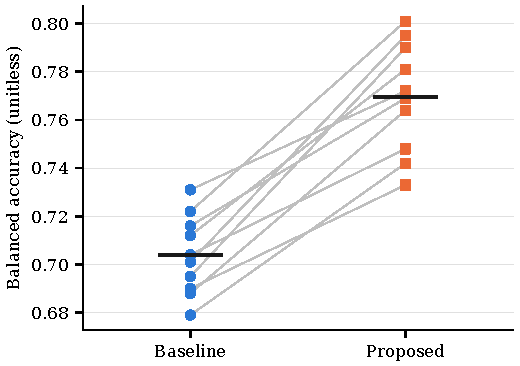
\includegraphics[width=\ifdim\linewidth<88mm \linewidth\else 88mm\fi]{Figure_2.pdf}
\caption{Balanced accuracy of the baseline and the proposed method on the same
\sonuc{kat.n} subject-wise folds. Each grey line joins the two results of one fold; the
thick bars are the means.}
\label{fig:paired}
\end{figure}
%% Şekil (Şekil 2): sekil_uret.py üretir -> sekiller/Figure_2.pdf (vektör PDF, basılı genişlik, 8 pt). Dosya numarası
%% PDF'teki şekil numarasıyla aynıdır (Şekil 1 blok diyagramdır). \graphicspath (ortak_baslik.tex) sayesinde şekil hem
%% sekiller/ klasöründe hem kökte bulunur. Altyazı tek başına anlaşılır: ne çizildi, kaç ölçüm, çizgi/çubuk ne demek.
%% Şekil içinde başlık yazılmaz. Bir başarılı ve bir başarısız örneği yan yana göstermek hakemin sorusunu önler.
%% Şekil ve görüntü yapay zekâya ürettirilmez ya da değiştirtilmez; yalnız çizim kodu düzelttirilebilir. Düzelttirdiyseniz beyan edilir:
%%   Elsevier'de diyagramın altyazısına, veri grafiğinde Methods'a aracın adı, sürümü ve geliştiricisi; IEEE'de Acknowledgment'a; HAFTA 5-A.
%% Görüntü lisansı ve kimlik kuralı: HAFTA 5-A.

\subsection{Sensitivity to one design choice}
%% En az BİR parametreyi (filtre bandı, pencere, eşik ...) değiştirip ana sonucun oynayıp oynamadığını
%% gösteriniz. "Neden komşu değer değil?" sorusunun cevabı buradadır. Yapmadıysanız bu alt bölümü SİLİNİZ
%% ve Limitations'a yazınız; yapılmamış işi yapılmış gibi yazmayınız.
\emph{(To be written from your own runs.)} Report how the main result changes when one
setting of Table~\ref{tab:params} is varied.

%% ---------------------------------------------------------------------------
%% 4 DISCUSSION  (HAFTA 4-B)   ~600-900 kelime
%% Üç paragraf: (1) sonuçlar ne anlama geliyor (tekrar değil, yorum)  (2) 2-3 atıflı çalışmayla
%% uyum/ayrılık  (3) bir mühendis/klinisyen bu sonuçla ne yapar. Sonra Limitations alt bölümü.
%% YORUM SİZİNDİR: önce kendi notlarınızı yazınız; sohbet yalnız notlarınızı İngilizce cümleye çevirir.
%% ---------------------------------------------------------------------------
\section{Discussion}
\label{sec:discussion}
%% HAFTA 4-B: önce kendi yorum notlarınız; sohbet yalnız İngilizceye çevirir ([BENİM YORUMUM YOK]).

Under a subject-wise protocol the simple classifier kept a consistent advantage over the
single-feature rule, whereas its difference from the re-run published method was not resolved:
the interval of that difference includes zero (Table~\ref{tab:main}). Subject-wise splitting
is the protocol recommended for clinical prediction problems~\cite{Saeb2017}; record-wise
splitting was not evaluated here, so the size of its optimistic bias on these data remains
unknown. The absolute values are not comparable with challenge
rankings~\cite{Clifford2016,Reyna2023}, which used hidden test sets and different scores.
%% Dil kanıta uygun olsun: "proves", "clearly", "significantly better" (testsiz) yazmayınız.
%% İlişki gösterdiyseniz "is associated with"; neden-sonuç demek için yalnız o şeyi değiştirmiş olmalısınız.

\subsection{Limitations and threats to validity}
\label{sec:limits}
\emph{Data:} a subset of one database; recordings from other devices were not tested.
\emph{Protocol:} one random assignment of subjects to folds. \emph{Methods:} one published
method was re-run; no deep model was included. \emph{Statistics:} fold-wise results share
training data, so the interval and the test are approximate; \sonuc{kat.n} folds give a coarse
estimate of variability. \emph{Use:} the study does not evaluate clinical benefit.
%% Tek liste, 5-8 kısa madde (veri, protokol, yöntem, istatistik, genelleme, kullanım, iç ve dış geçerlilik); her maddeye
%% bir sonraki adım cümlesi ekleyiniz. Hakemden ÖNCE siz yazınız.

%% ---------------------------------------------------------------------------
%% 5 CONCLUSION  (HAFTA 4-B)   tam İKİ paragraf, ~200-300 kelime, yeni sonuç ve atıf YOK
%% 'improved ... by \sonuc{fark.ort}': düşük değeri iyi olan metrikte fark eksidir; 'reduced the error by' gibi yön kelimesi seçiniz.
%% ---------------------------------------------------------------------------
\section{Conclusion}
\label{sec:conclusion}

On \sonuc{kat.n} subject-wise folds of open heart sound data, a logistic-regression
classifier improved balanced accuracy over a single-feature rule by \sonuc{fark.ort} on
average, under the conditions listed in Table~\ref{tab:params}.

Future work will repeat the comparison on a second database and vary the filter band to test
how far the result generalises.


%% ============================================================================
%% BEYANLAR (HAFTA 5-A). Başlıkların ADI ve SIRASI derginin kılavuzundan alınır; hepsi DOĞRU olmalıdır.
%% ============================================================================
\section*{CRediT authorship contribution statement}
\textbf{Ad Soyad:} Conceptualization, Methodology, Software, Formal analysis, Writing -- original draft.
\textbf{Danışman Ad Soyad:} Supervision, Writing -- review \& editing.
%% Roller CRediT listesinden seçilir; yalnız GERÇEKTEN yapılan roller yazılır.

\section*{Declaration of competing interest}
The authors declare that they have no known competing financial interests or personal
relationships that could have appeared to influence the work reported in this paper.

\section*{Funding}
This research did not receive any specific grant from funding agencies in the public,
commercial, or not-for-profit sectors.
%% Destek varsa (ör. TÜBİTAK 2209-A) kurum adı ve proje numarası yazılır; yoksa yukarıdaki cümle kalır.

\section*{Ethics statement}
This study used only publicly available, de-identified recordings~\cite{Oliveira2022data},
distributed under the Open Data Commons Attribution License~v1.0; no new data were collected
from human participants, and ethical approval was therefore not required. The original data collection
was approved by an institutional review board, and participants younger than 21 years were included with a signed
parental consent form where appropriate, as described with the dataset~\cite{Oliveira2022data}.
%% Bu son cümleyi yalnız veri setinin sayfası ya da tanıtım makalesi bunu yazıyorsa bırakınız (CirCor için PhysioNet sayfasının
%% Methods ve Ethics bölümleri yazıyor, 14.11.2026'da okundu); yazmıyorsa "consent was not obtained by the authors because the
%% data are public and de-identified" deyiniz.
%% Lisansın ADI veri setinin kendi sayfasından okunur; kendi verinizinkini yazınız (tahmin etmeyiniz).
%% Verinin özgün toplanışındaki etik onay ve onam, veri tanıtım makalesinde yazıyorsa ona atıf veriniz.
%% KENDİ kaydınızı aldıysanız bu cümle YANLIŞ olur: etik kurul adı, karar numarası ve
%% aydınlatılmış onam yazılmak zorundadır. Etik onay yoksa açık veri kullanınız.

\section*{Data and code availability}
The recordings (version~1.0.3) are available from PhysioNet~\cite{Oliveira2022data,Pollard2026}
under the Open Data Commons Attribution License~v1.0 and are not redistributed with this paper.
The code, the results file and the scripts that produce all reported values and figures are
available at \url{https://github.com/kullanici/depo} (tag \texttt{v1.0}).
%% Veri SÜRÜMÜ ve LİSANSI yazılır. Ham veri setini deponuza YÜKLEMEYİNİZ: kaynağına link verip atıflayınız;
%% depoda yalnız kodunuz ve sonuç dosyanız durur. Kimlik taşıyan bilgi (DICOM üstverisi, yüz, ad, tarih)
%% makaleye ve depoya girmez. Kayıt ya da sözleşme isteyen veride sözleşmenin paylaşım koşullarını okuyunuz.
%% Makaleye görüntü koyuyorsanız lisansı yayına izin vermeli ve kaynağı altyazıda yazılmalıdır.
%% Depo linki ve etiketi (tag) GERÇEK olmalıdır; etiket, sonuçları üreten sürümü gösterir.

\section*{Declaration of generative AI and AI-assisted technologies in the manuscript preparation process}
During the preparation of this work the authors used [TOOL NAME, version] to turn the authors'
own notes, code and results into English draft text for the Introduction, Methods, Results and
Discussion; to suggest wording for the title, abstract, keywords, highlights and figure captions;
to correct the authors' plotting and diagram code; and to adapt the authors' results script. The
tool did not produce data, numbers, references, figures or interpretations. After using this
tool, the authors reviewed and edited the content as needed and take full responsibility for the
content of the published article.
%% Bu beyan DOĞRU ve EKSİKSİZ olmalıdır: sohbete hangi bölümde ne yaptırdıysanız onu yazınız; yaptırmadığınızı siliniz.
%% Bu derste herkes sohbet kullandığı için "yalnız dil düzeltmesi" cümlesi YANLIŞTIR.
%% Kod ve betik yardımını Methods'ta da bir cümleyle anınız (Elsevier: araştırmada kullanılan yapay zekâ Methods'ta yazılır).
%% Elsevier şekil kuralı: yapay zekâ desteği alan diyagram altyazısında, veri grafiği Methods'ta aracın adı, sürümü ve geliştiricisiyle
%% beyan edilir; araştırma görüntüsü yapay zekâyla üretilmez ya da değiştirilmez. Bu derste şekil ve görüntü yapay zekâya
%% ürettirilmez; yalnız sizin çizim kodunuz düzelttirilebilir. Başlık metni derginin kılavuzundaki ile birebir aynı olmalıdır.

\bibliographystyle{elsarticle-num}
\bibliography{refs}

\end{document}
